\documentclass[conference]{IEEEtran}
\usepackage{hyperref}

\IEEEoverridecommandlockouts
% The preceding line is only needed to identify funding in the first footnote. If that is unneeded, please comment it out.
\usepackage{cite}
\usepackage{amsmath,amssymb,amsfonts}
\usepackage{algorithmic}
\usepackage{graphicx}
\usepackage{textcomp}
\usepackage{xcolor}

\usepackage{subfigure}
\usepackage{tikz}
\usepackage{pgfplots}

\newcommand{\dprobtf}{\ensuremath{\mathsf{DPRobTF}}}

\def\BibTeX{{\rm B\kern-.05em{\sc i\kern-.025em b}\kern-.08em
    T\kern-.1667em\lower.7ex\hbox{E}\kern-.125emX}}
    
\usepackage{amsthm}
\theoremstyle{definition}
\newtheorem{definition}{Definition}
\newtheorem{theorem}{Theorem}
    
\begin{document}

%\title{SAT Encoding for the Robust Team Formation Problem}
\title{SAT Benchmarks for the Robust Team Formation Problem}

\author{
	\IEEEauthorblockN{Nicolas Schwind}
	\IEEEauthorblockA{
		\textit{National Institute of Advanced}\\ 
		\textit{Industrial Science and Technology} \\
		Tokyo, Japan\\
		nicolas-schwind@aist.go.jp
	}
	\and
	\IEEEauthorblockN{Emir Demirovi\'c}
	\IEEEauthorblockA{
		\textit{~~~~~~~~~~~~~~~~~~Delft University of Technology~~~~~~~~~~~~~~~~~~~}\\ 
		Delft, The Netherlands\\
		e.demirovic@tudelft.nl\\
	}
	\and 
	\IEEEauthorblockN{Katsumi Inoue}
	\IEEEauthorblockA{
	\textit{National Institute of Informatics} \\
	\textit{~~~~~~The Graduate University for Advanced Studies, SOKENDAI}\\
	Tokyo, Japan\\
	inoue@nii.ac.jp
	}	
	\and
	\IEEEauthorblockN{Jean-Marie Lagniez}
	\IEEEauthorblockA{
	\textit{Universit\'e d'Artois} \\
	\textit{CRIL-CNRS}\\
	Lens, France\\
	lagniez@cril.fr
	}
}


\maketitle

\begin{abstract}
Team formation (TF) is the problem of deploying the least expensive team of agents 
while covering a set of skills. It is almost equivalent to the Set Cover problem.
Robust team formation (RobTF), a generalization of TF,
takes into account the dynamic nature of the environment. Indeed, after 
a team has been formed, agents may unexpectedly become unavailable
due to failure or illness.
A team is said to be $k$-robust if it still covers the set of skills even after $k$ agents are removed from it.
%Thus it is equivalent to TF for $k=0$.
Robustness is clearly a desirable property as it allows the underlying system to remain 
functional after an unfortunate event occurs.
The decision problem for RobTF consists, given two integers $k, b$, in finding a $k$-robust team whose deployment cost is not greater than
$b$. Interestingly, this problem is $\mathsf{NP}$-complete,
%for any integer $k$,
making it an appropriate target for SAT solvers.
\end{abstract}

\begin{IEEEkeywords}
team formation, SAT encoding.
\end{IEEEkeywords}

\section{Introduction}

Team Formation (TF) consists in forming a team of agents with minimum cost so as 
to meet a certain set of requirements. 
We are given a set of agents, where each agent is associated with a set of skills and a 
deployment/hiring cost. The TF problem consists in finding a team $T$ 
(i.e., a subset of agents) of minimal overall cost that is \emph{efficient}, i.e.,
such that each skill is possessed by at least one agent from $T$. 
This is an important problem in multi-agent systems and has been studied in the 
contexts of RoboCup rescue teams \cite{DBLP:journals/aim/KitanoT01}, 
unmanned aerial vehicle operations \cite{DBLP:conf/atal/GeorgePSS10}, 
social networks \cite{KargarAZ12,FarhadiHHH12}, 
online football prediction games \cite{MatthewsRC12}, among others. 
This problem is well-known to be NP-hard \cite{DBLP:books/fm/GareyJ79,Okimoto2015}.
The (standard) TF problem \cite{Okimoto2015} can be formally defined as follow:

\begin{definition}[TF Problem Description]
	A \textit{TF problem description} is a tuple $\langle A, S, f, \alpha\rangle$ 
	where $A = \{a_1, \ldots ,a_n\}$ is a set of agents, $S = \{s_1, \ldots, s_m\}$ is a set of 
	skills, $f : A \mapsto \mathbb{N}$ is a deployment cost function, and $\alpha : A \mapsto 2^S$ is an agent-to-skill function.
	\label{def:TFpd}
\end{definition}

A \emph{team} is a subset of agents $T \subseteq A$.
One extends the cost function $f$ to teams $T$ as $f(T) = \sum_{a_i \in T}{f(a_i)}$.
Likewise, the agent-to-skill function $\alpha$ is extended to teams $T$
as $\alpha(T) = \bigcup_{a_i \in T}{\alpha(a_i)}$.
A standard expected property in Team Formation is efficiency:
a team $T \subseteq A$ is \emph{efficient} if all skills from $S$ are covered
by $T$, i.e., when $\alpha(T) = S$.  An optimal team for TF is an
efficient team minimizing the cost function.  The corresponding decision
problem asks, given a TF problem description and a
bound $b \in \mathbb{N}$ as input, whether there exists an
efficient team $T$ such that $f(T) \leq b$.  This problem is
equivalent to the well-known set cover problem
\cite{DBLP:books/fm/GareyJ79} and is $\mathsf{NP}$-complete \cite{Okimoto2015}. \\


In realistic settings, we may not be certain about the actual functionality of 
all agents from a team after
%computation and
deployment.
Some unexpected, exogenous events often occur:
agents get sick or may be unable to do the job for various reasons,
and we may mot be certain about the actual functionality of all agents from a team 
after
%formation and
deployment. Thus it is important to consider \emph{robustness} properties in TF,
i.e., seek to form an efficient team that is proactive to such unfortunate changes.

%, i.e., it remains efficient 
%even when some agents are removed from the deployed team.
The notion of robustness in Team Formation has been introduced and formalized in \cite{Okimoto2015}:
\begin{definition}[Robust Team \cite{Okimoto2015}]
	Given a TF problem description $\langle A, S, f, \alpha\rangle$ and  $k \in \mathbb{N}$, a team $T$
	is said to be \emph{$k$-robust} if for every set of agents $T' \subseteq T$ such that $|T'| \leq k$, the team $T \setminus T'$ is efficient.
	\label{def:TFrobust}
\end{definition}

\begin{figure*}
	\centering
	\begin{minipage}{.19\textwidth}
		\centering
		
\includegraphics[width=\textwidth]{tf-a}
	\end{minipage}
	\begin{minipage}{.19\textwidth}
		\centering
		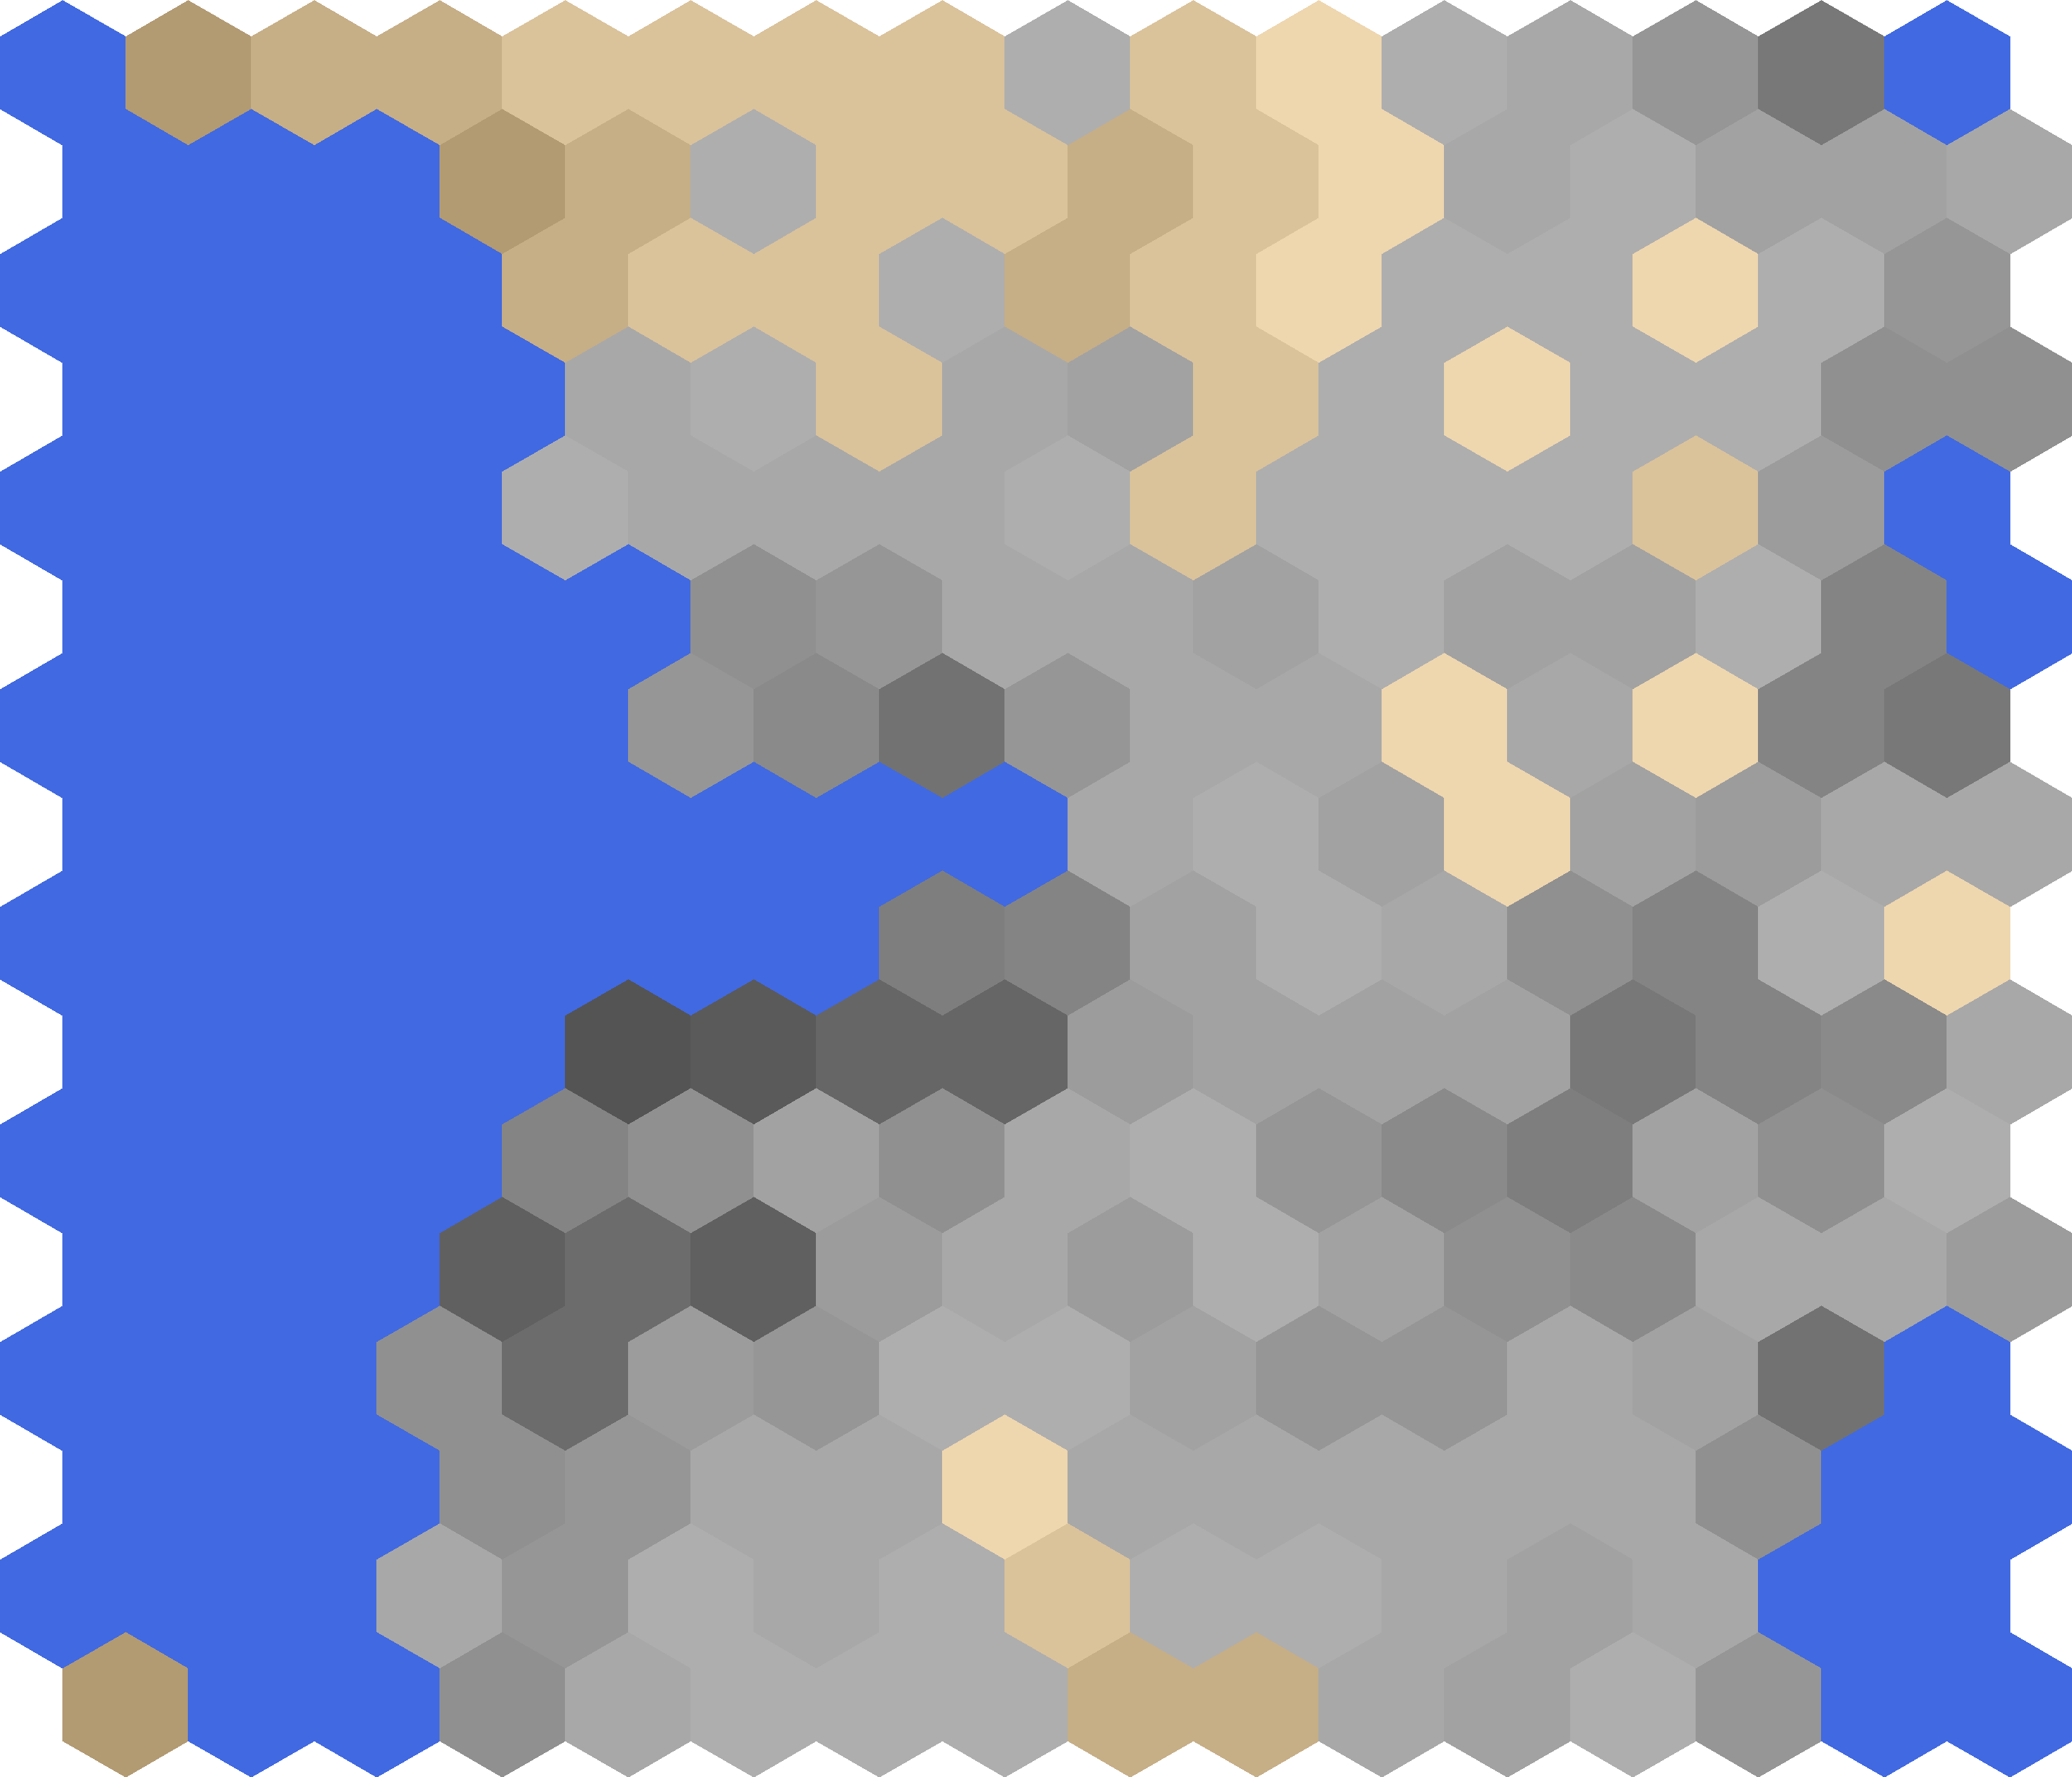
\includegraphics[width=\textwidth]{tf-b}
	\end{minipage}
	\begin{minipage}{.19\textwidth}
		\centering
		
\includegraphics[width=\textwidth]{tf-c}
	\end{minipage}
	\begin{minipage}{.19\textwidth}
		\centering
		
\includegraphics[width=\textwidth]{tf-d}
	\end{minipage}
	\begin{minipage}{.19\textwidth}
		\centering
		
\includegraphics[width=\textwidth]{tf-e}
	\end{minipage}
	
	\begin{minipage}{.19\textwidth}
		\centering
		
\includegraphics[width=\textwidth]{tf-f}
	\end{minipage}
	\begin{minipage}{.19\textwidth}
		\centering
		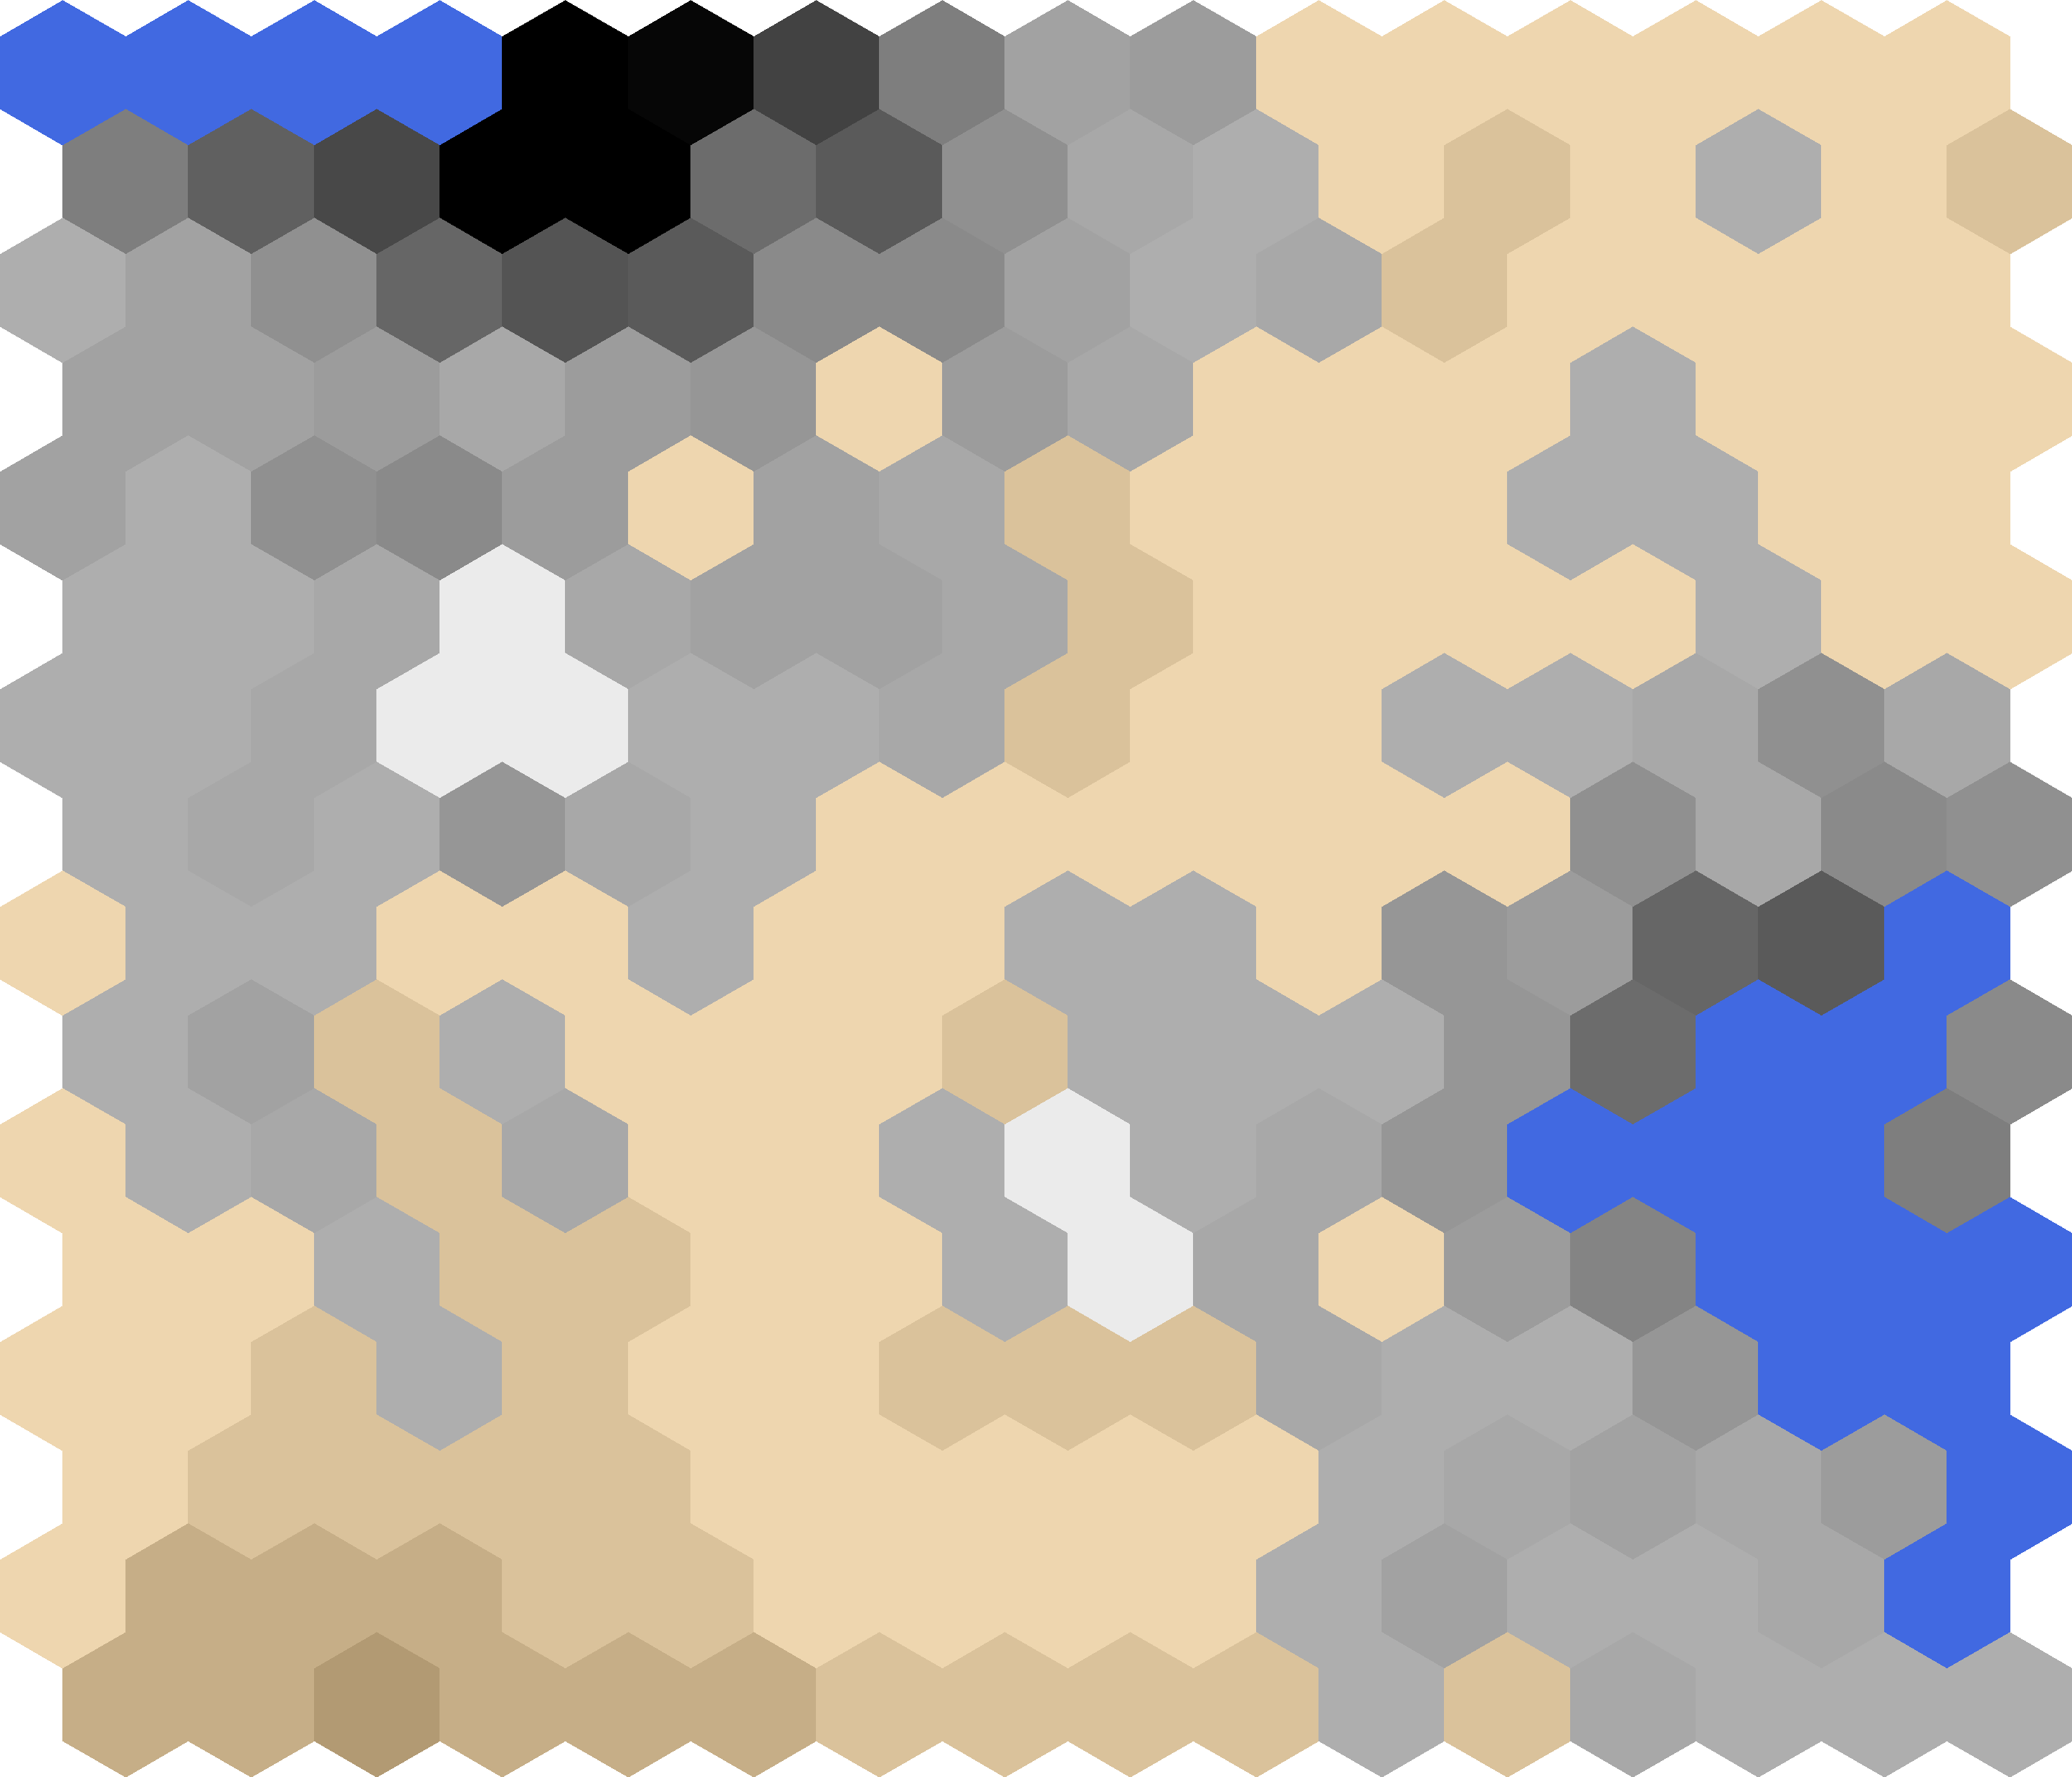
\includegraphics[width=\textwidth]{tf-g}
	\end{minipage}
	\begin{minipage}{.19\textwidth}
		\centering
		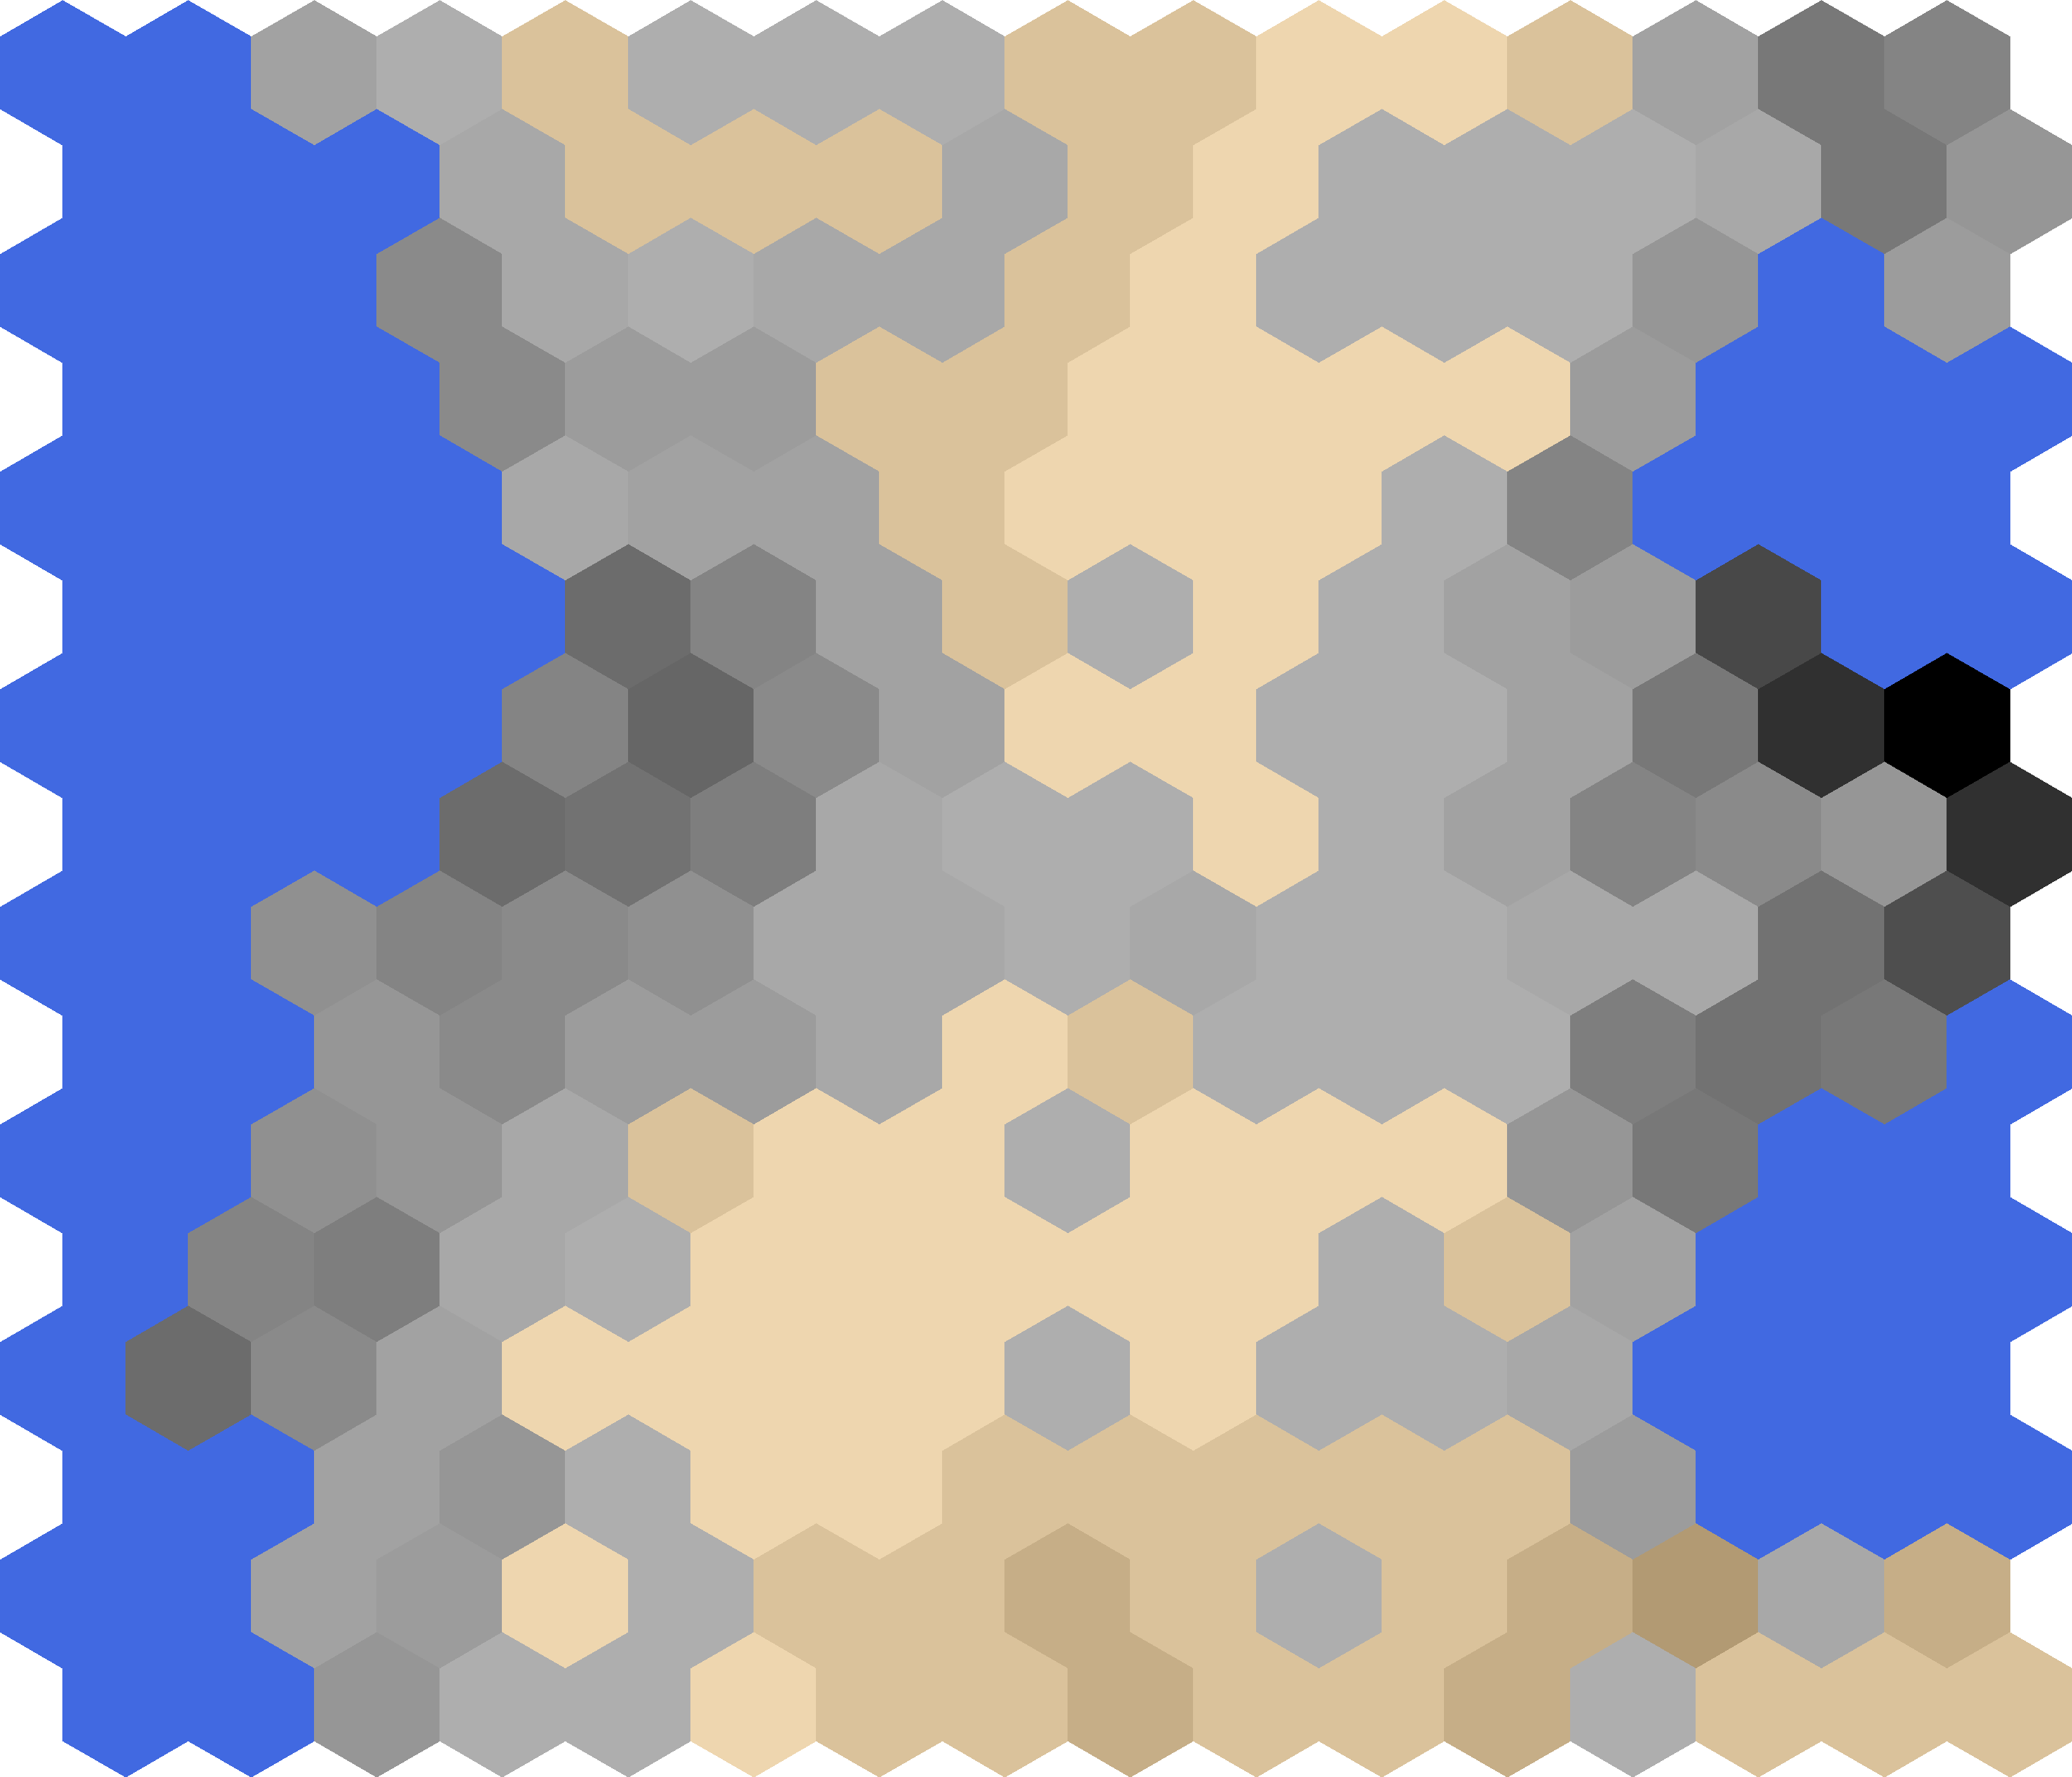
\includegraphics[width=\textwidth]{tf-h}
	\end{minipage}
	\begin{minipage}{.19\textwidth}
		\centering
		
\includegraphics[width=\textwidth]{tf-i}
	\end{minipage}
	\begin{minipage}{.19\textwidth}
		\centering
		
\includegraphics[width=\textwidth]{tf-j}
	\end{minipage}
	\caption{Some examples of populated maps.}
	\label{fig:mapsss}
\end{figure*}

Indeed, a team $T$ is $k$-robust if it remains efficient in any
case where at most $k$ agents are removed from it.
Robust TF (RobTF) consists in finding an optimal $k$-robust team, i.e., a
$k$-robust team of minimal deployment cost. It provides a
guarantee that the goal is fulfilled in the worst case given $k$.
Robustness generalizes efficiency: a team is $0$-robust if and only if it is efficient.
%This involves introducing redundant agents which may not be necessary if the worst case does not happen.
Interestingly,
%computing an optimal robust team is not harder than computing an optimal
%efficient team \cite{Okimoto2015}, since
checking whether a team is $k$-robust only requires to
check that every skill is covered at least $k + 1$ times \cite{Okimoto2015}, and this can be done in polynomial time.
%Formally, we have:
%The generalization is strict, since higher values of $k$ lead to different optimal teams \cite{Okimoto2015}.
Hence, despite this generalization, finding an optimal $k$-robust team (for any $k \geq 0$) does not lead to a computational shift
compared to finding an optimal efficient team. Let us formalize the decision problem for RobTF, which is the problem of interest here:
\begin{definition}[\dprobtf]\hfill
	\begin{itemize}
		\item[$\bullet$] \textbf{Input:} A TF problem description, two integers $k, b$.
		\item[$\bullet$] \textbf{Question:} Does there exist a $k$-robust team $T \subseteq A$ such that $f(T) \leq b$?
	\end{itemize}
	\label{def:decision problem}
\end{definition}
%Indeed, the decision problem for robustness, which asks, given a TF problem description and $c, k$ in $\mathbb{N}$,
%if there exists a $k$-robust team $T \subseteq A$ such that $f(T) \leq c$, is $\mathsf{NP}$-complete.
%Indeed, the decision problem for robustness (labeled \DPRobTF) asks, given a TF problem description and $c, k$ in $\mathbb{N}$,
%if there exists a $k$-robust team $T \subseteq A$ such that $f(T) \leq c$. Then:

\begin{theorem}[\cite{Okimoto2015}]
	\dprobtf{} is $\mathsf{NP}$-complete.
	\label{prop:TORTF}
\end{theorem}


\section{Robust Facility Deployment}

\newcommand\widthmap{.3}
\begin{figure*}[tp]
	\centering
	\subfigure[A populated map generated by our procedure.]{
		\label{subfig:map-alone}
		
\includegraphics[width=\widthmap\textwidth]{TF-1}
	}\quad
	\subfigure[An optimal $0$-robust team $T_1$ ($f(T_1) = 20$, $rc(T_1, 1) = 13$, $pc(T_1, 1) = .20$).]{
		\label{subfig:map-solutionTF}
		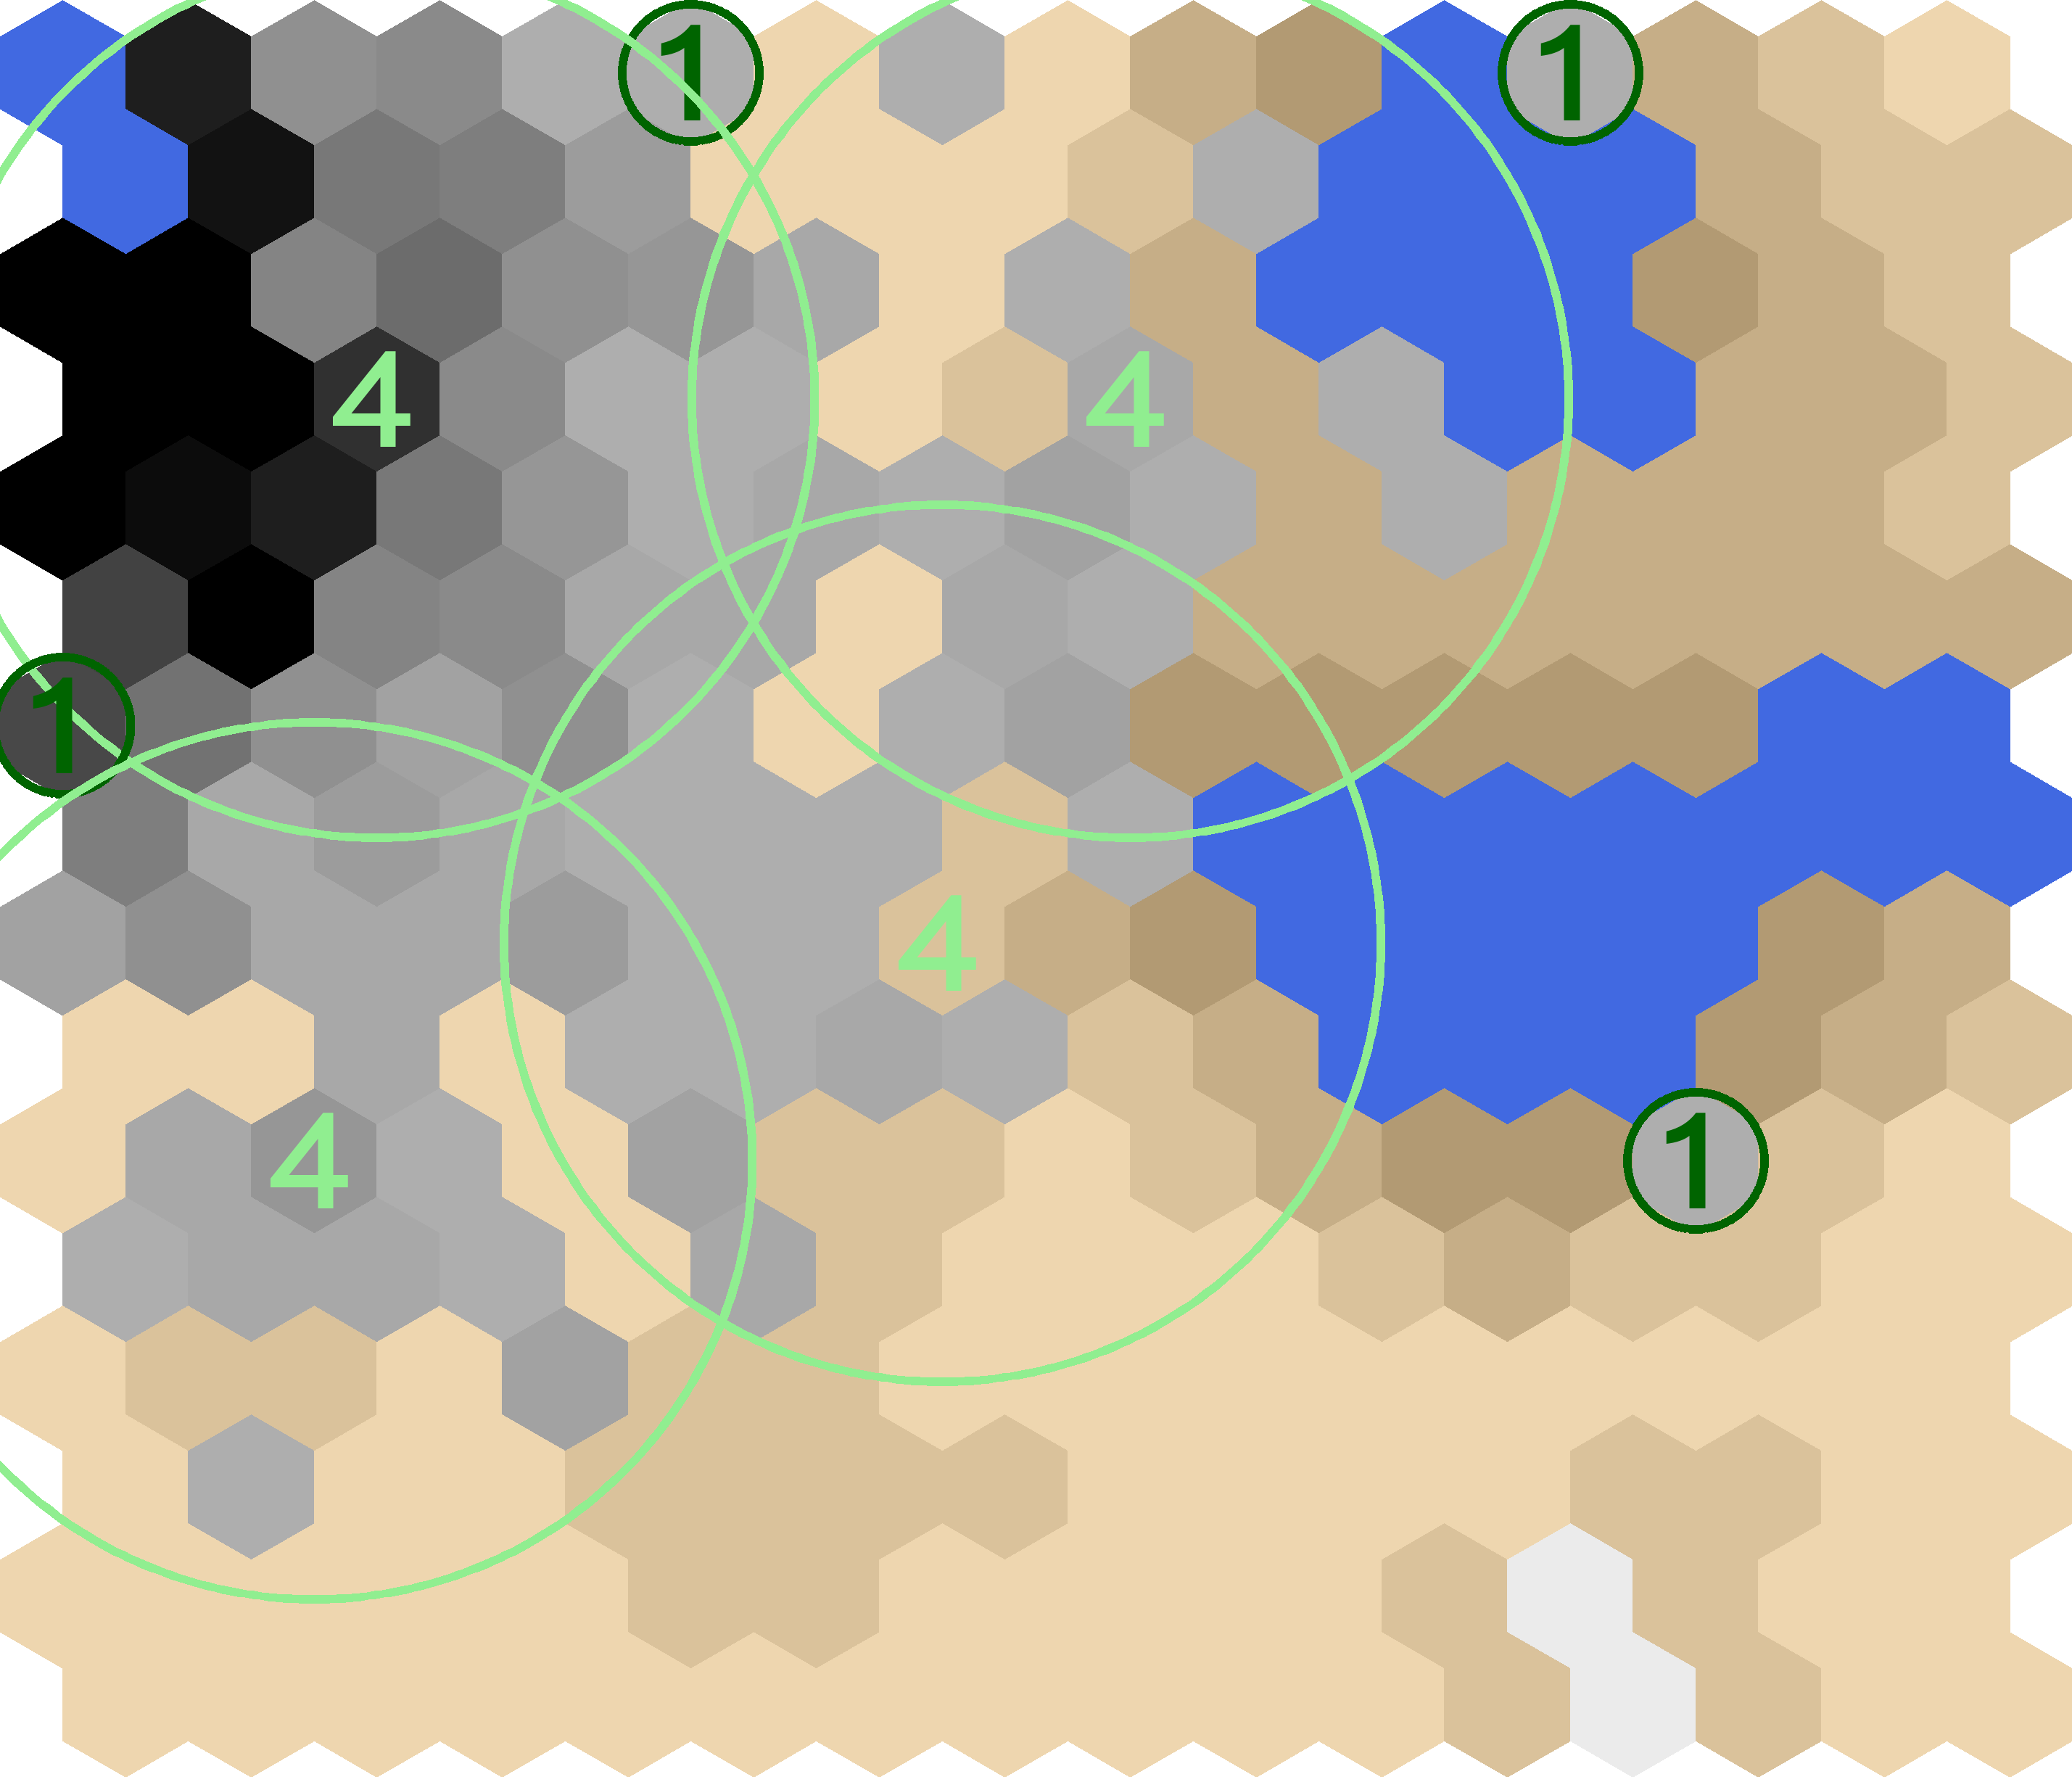
\includegraphics[width=\widthmap\textwidth]{TF-1-TF}
	}\quad
	\subfigure[An optimal $1$-robust team $T_2$ ($f(T_2) = 41$, $rc(T_2, 1) = 0$, $pc(T_2, 1) = 1$).]{
		\label{subfig:map-solutionKTF}
		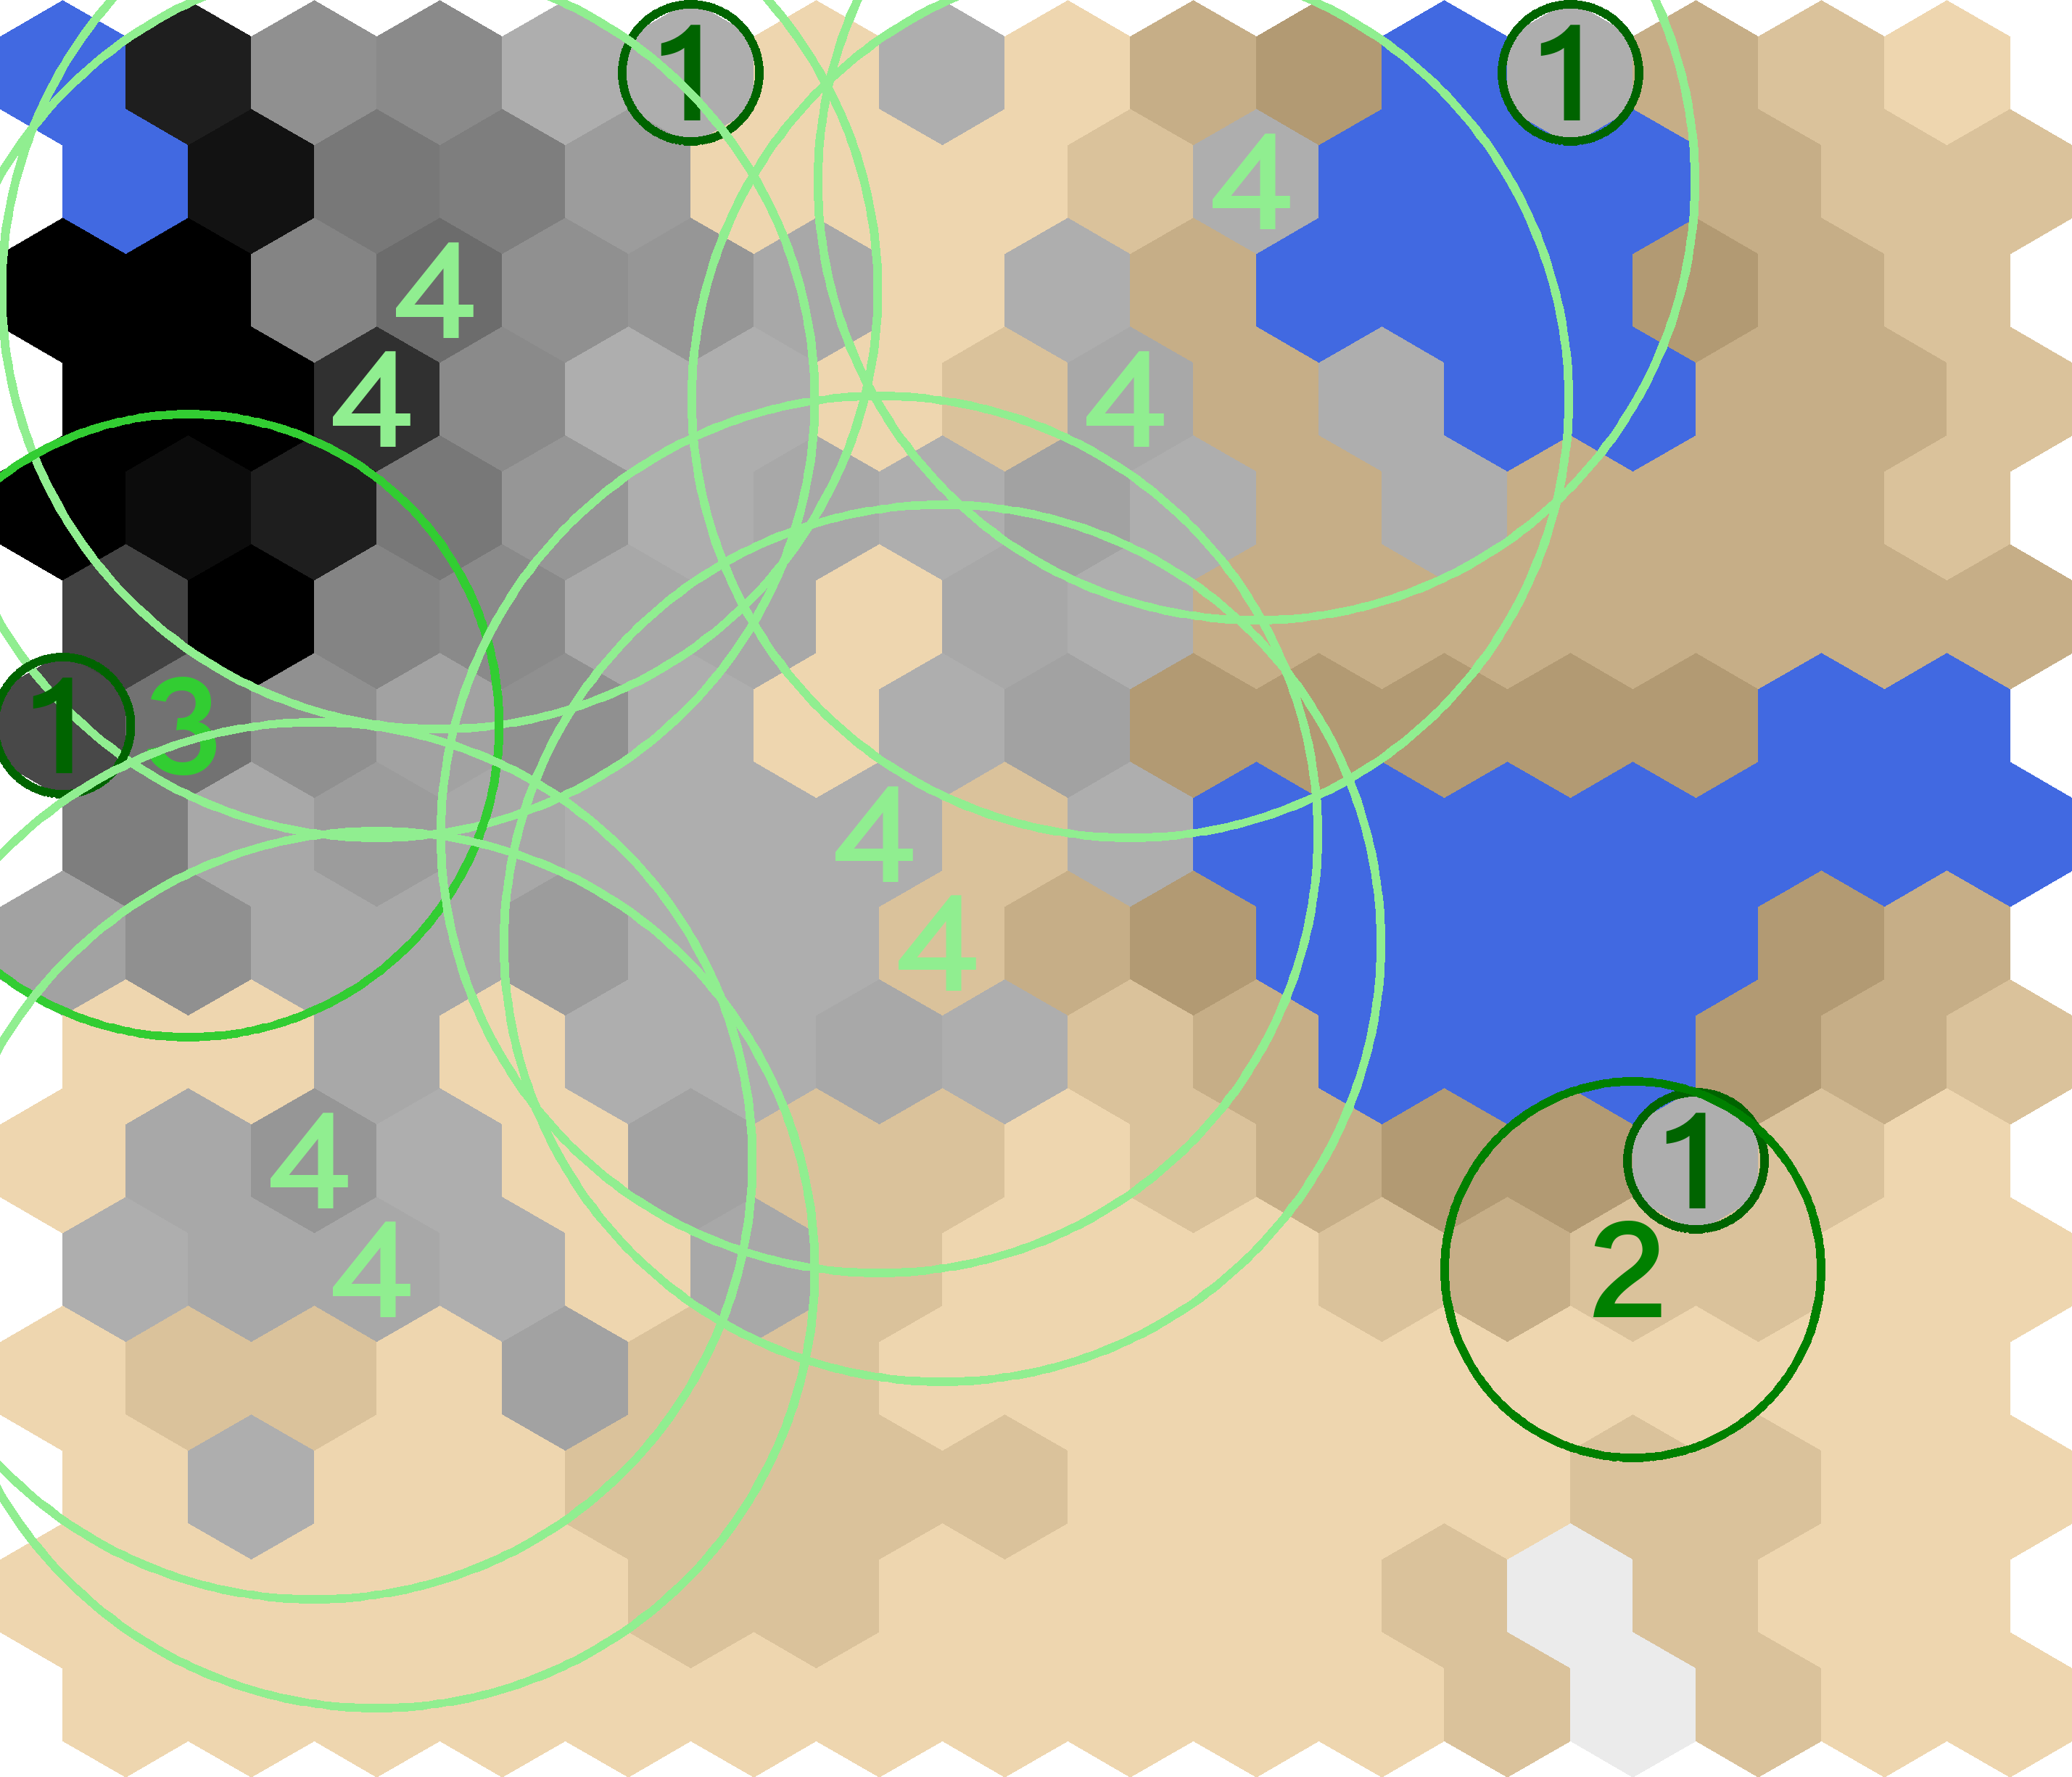
\includegraphics[width=\widthmap\textwidth]{TF-1-KTF-k1}
	}
	\caption{Optimal 0-robust and 1-robust teams for a given instance.}
	\label{fig:map-solution}
\end{figure*}

In \cite{schwind2021}, we have introduced
%a new solution concept for Team Formation, together with
a generator of TF problem descriptions
%which turns out to be a compromise between robustness and resilience \cite{schwind2016,demirovic2018}.
%we artificially generate instances
modeling facility deployment problem instances.
This problem consists in deploying a set of facilities 
(e.g., health centers, antennas, schools, shelters) on a populated map
so as to maximize a certain population coverage while minimizing the overall deployment cost \cite{fac}.
The problem is of particular importance, e.g., for mobile phone operators
which aim to deploy a set of cell towers in an urban environment.
Finding an optimal efficient team allows one to find a facility deployment
of minimal cost while providing a service coverage over
the whole population.
In such an application context, each populated cell corresponds to a skill to be covered,
each facility at a given location corresponds to an agent,
and the skills associated with a facility are the populated cells in its range.
%\footnote{In these instances, the skill is associated with a ``weight'' which
%corresponds to the density of the population at that location \cite{schwind2021}. However, that weight is not relevant for the problem
%considered here, so it is .}
%(the weight depends on the density of the population at a precise location).
Each TF problem instance was synthesized following three steps.

First, one generates an elevation map made of water parts, lands and mountains. 
A 16x16 grid of numbers is created using
Perlin noise \cite{perlin}, a procedural texture primitive commonly used by visual 
effects artists to increase the appearance of realism in
computer graphics. The grid is then converted into a hexagonal grid for which each cell is associated with
a ``type'' depending on the range of its value according to the grid.
A low (resp., mid, high) value is interpreted as a water cell (resp., a mountain cell, a land cell).

Second, the map is populated by iteratively adding an individual on the grid. 
Initially, three individuals are added in three different land cells randomly chosen,
provided that the cell is next to a water cell. Then, a new individual is added at 
random following a probability distribution.
The water cells and the cells that already host 10 individuals cannot host a new individual.
Among the remaining cells, the closer to a densely populated cell or to water cell,
the higher its probability to welcome a new individual.
The process is repeated 600 times which at last corresponds to the total 
population in the map.
%Fig.~\ref{subfig:map-alone} represents a populated map
Fig.~\ref{fig:mapsss} depicts ten populated maps
generated using
this method: blue (resp. white, brown) cells are of water type (resp. mountain, field type).
The scales of brown correspond to different elevation degrees of land.
The scales of gray represent the number of individuals in a cell: the darker a cell,
the more densely populated, so a pitch black cell contains 10 individuals.
The different scales of brown/gray do not have an impact on the final TF instance, but were
%correspond to different elevation degrees of land, only 
used to tune the probability of adding an individual to a land cell, so that to make the instance more realistic.
%Figure~\ref{fig:map-examples} depicts some examples of generated map instances using our method.
%The gray scales represent the number of individuals in a cell. 
%The darker a cell, the more densely populated, so 

Third, a populated map is translated into a weighted TF problem description
 $\langle A, S, f, \alpha\rangle$ as follows.
We consider four types of agents $type_1, \ldots, type_4$. 
Each type $type_i$ of agent corresponds to a facility that has a deployment cost
equal to $i$ and a cover range equal to $i - 1$. For instance, a cell tower 
of type $type_3$ has a deployment cost equal to $3$, and when it is
deployed in a certain cell $C$ on the grid, it provides the required service 
to anyone that is in a cell $C'$ where the distance between
$C$ and $C'$ is at most $2$; the distance between two cells on the grid corresponds 
to the length of the shortest path
between $C$ and $C'$. So for each type of facility $type_i$ and each grid cell $j$ that is not of water type,
one considers an agent $a_i^j$ of cost $f(a_i^j) = i$ which corresponds to a 
facility of type $type_i$ to be potentially deployed in the cell $j$.
This defines the set $A$ of agents and the cost function $f$.
To define the set of skills $S$,
one simply associates each populated grid cell $p$ 
(i.e., a cell that hosts at least one individual) with a skill $s_p$.
%and the skill weight function $w_\Sigma$ 
%(note that we considered a normalized weighted sum function)
%are simply defined as follows. One associates with each populated grid cell $p$ 
%(i.e., a cell that hosts at least one individual) a skill $s_p$; and the weight 
%of each skill $w_\Sigma(s_p)$ is defined as the number of individuals in the grid cell $p$.
Lastly, the agent-to-skill mapping $\alpha$ is defined as follows. An agent $a_i^j$ 
has the skill $s_p$ if the grid cell $p$ is within the reach of the facility $a_i^j$, 
i.e., if the distance between the grid cells $j$ and $p$ is less than or equal to $i - 1$.
The generated instances were formed of 500 to 700 agents and 50 to 150 skills.


Given such an instance $\langle A, S, f, \alpha\rangle$, a team $T$ 
corresponds to a set of facilities to be deployed on the corresponding map.
Fig.~\ref{fig:map-solution} depicts for a given map instance the optimal team computed, that is
respectively $0$-robust, or equivalently, efficient (Fig. \ref{subfig:map-solutionTF}) and $1$-robust (Fig. \ref{subfig:map-solutionKTF}).
For instance, the optimal $0$-robust team (Fig. \ref{subfig:map-solutionTF}) 
is formed of eight agents corresponding to four facilities
of type $type_4$ and four facilities of type $type_1$. Each such facility 
is represented by a label on the corresponding grid cell
ranging from $1$ to $4$, corresponding to its type / deployment cost. 
The circle drawn around each deployed facility represents the populated area
that is covered by it, i.e., the set of skills possessed by the corresponding agent.
%Let us remark that in the context we are interested in $w_\Sigma$ is not relevant since
%we search a team that satisfies all the skills. The case where $w_\Sigma$ is relevant 
%concerns other team formation behaviour that are out of the scope of this system description
%(interested readers can refer to \cite{schwind2021} for other team formation behaviour).

\section{SAT Encoding}

We are interested in formalizing the decision problem \dprobtf{} given in Definition~\ref{def:decision problem}
as a SAT problem.
%a bound $b \in \mathbb{N}$ is considered.
%The objective is then to find out a team such that its computed cost is less than $b$.
%To translate our problem into SAT
To do so, we first associate a boolean 
variable $p_i$ with each agent in $a_i \in A$, where $p_i$ is true
if and only if the agent $a_i$ is present in the deployed team.
%In the following we describe the encoding for the $k$-robust case, the efficient
%case beeing the special case where $k=0$.
The encoding is described as follows.
Given a TF instance $\langle A, S, f, \alpha\rangle$ and $k, b \in \mathbb{N}$,
a $k$-robust team $T$ exists if and only if:
\begin{equation}
\bigwedge_{s_j \in S} \sum_{a_i \in A | s_j \in \alpha(i)} p_i > k
\end{equation}

\begin{equation}
\sum_{a_i \in A} f(i) \times p_i \leq b
\end{equation}

Equation~1 ensures that at least $k + 1$ agents present in the deployed team the team.
This equation precisely ensures that the team is $k$-robust \cite{Okimoto2015}.
%i.e., that at least $k + 1$ agents present in the deployed team.
It consists in a set of cardinality constraints encoded into CNF using PySAT \cite{imms-sat18}.
In the case where $k = 0$, the cardinality constraints are encoded as clauses. 
For the general case where $k > 0$ the cardinality constraints are encoded into SAT using
the totalize encoding \cite{BailleuxB03}.
Equation~2 ensures that the cost of the deployed team is not more than the bound $b$.
It consists in one pseudo-boolean constraint
that has been encoded into SAT using the encoding type \textit{best} provided by PySAT.

\section{Benchmarks}

We submitted 20 benchmarks to the 2021 SAT Competition.
The benchmarks are named as $ktf\_\langle bench.tf \rangle \_\langle k \rangle\_\langle ratio \rangle\_\langle b\rangle$, where:
\begin{itemize}
	\item $bench.tf$ is the TF instance used to generate the CNF formula,
	\item $k$ is requirement of $k$-robustness,
	\item $ratio$ is a ratio (a value between 0 and 1) of the overall cost the set of all agents, used to define the bound $b$; for instance,
	one sets a ratio of 0.6 when one wants the cost of the deployed team to be less than or equal to 60\% of the total cost of all agents.
	\item $b$ is the bound defined as $b = ratio \times \sum_{a_i \in A} f(a_i)$.
\end{itemize}


%follow the following naming convention:
%\begin{itemize}
%\item Efficient team: $tf\_\langle bench.tf \rangle \_\langle ratio \rangle\_\langle bound \rangle$, 
%where $bench.tf$ is the team formation input that has been used to generate the CNF formula,
%$ratio$ is a ratio of the maximum cost we can deployed, and $bound$ is the given bound 
%($bound = ratio \times \sum_{i \in A} f(i)$);
%\item $k$ robust team: $ktf\_\langle bench.tf \rangle \_\langle k \rangle\_\langle ratio \rangle\_\langle bound \rangle$, where $bench.tf$ is the team formation input that has been used to generate the CNF formula,
%$k$ is the maximal number of agents we can lose,
%$ratio$ is a ratio of the maximum cost we can deployed, and $bound$ is the given bound 
%($bound = ratio \times \sum_{i \in A} f(i)$);
%\end{itemize}

All the materials used to generate the benchmarks are available at \url{https://github.com/jm62300/team-formation}.


\bibliographystyle{IEEEtrans} 
\bibliography{teamFormation}



\end{document}
